\newcommand{\titleinfo}{Wavelets}
\newcommand{\subjectinfo}{From Fourier To Wavelets}
\newcommand{\authorinfo}{Gian Danuser, Roman Koller}
\newcommand{\versioninfo}{0.1}
\newcommand{\newpar}{\par\par}

%%%%%%%%%%%%%%%%%%%%%%%%%%%%%%%%%%%%%%%%%%
% Dokument
%%%%%%%%%%%%%%%%%%%%%%%%%%%%%%%%%%%%%%%%%%
\documentclass[11pt,twoside]{scrartcl} %oneside Change xxxside -->marginpar must bee changed

\usepackage[pdftitle={\titleinfo},%
						pdfauthor={\authorinfo},%
						pdfcreator={pdfLatex, LaTeX with hyperref},
						pdfsubject={\subjectinfo},
						plainpages=false,
						pdfpagelabels,
						colorlinks,
						linkcolor=black,
						filecolor=black,
						citecolor=black,
						urlcolor=black]{hyperref}
						

% Headings
\usepackage{fancyhdr}
\renewcommand{\headrulewidth}{0.4pt}
\renewcommand{\footrulewidth}{0.4pt}	

\lhead[\scriptsize\nouppercase{\leftmark}]{\textbf{\titleinfo}}
\chead[V\versioninfo]{V\versioninfo}
\rhead[\textbf{\titleinfo}]{\scriptsize\nouppercase{\leftmark}}

\lfoot[\thepage]{\authorinfo}
\cfoot[]{}
\rfoot[\authorinfo]{\thepage}


%%%%%%%%%%%%%%%%%%%%%%%%%%%%%%%%%%%%%%%%%%
% Package's
%%%%%%%%%%%%%%%%%%%%%%%%%%%%%%%%%%%%%%%%%%
\usepackage{ucs}
\usepackage[utf8x]{inputenc}
\usepackage[T1]{fontenc}

\usepackage{layout}
\setlength{\parindent}{0em}

\usepackage{lscape}

\renewcommand{\baselinestretch}{1.2}
\renewcommand{\arraystretch}{1}

%Damit \today ein Deutsch Formatiertes Datum zurueckgibt.
\usepackage[ngerman, num, orig]{isodate}
\usepackage[german, ngerman]{babel}
\monthyearsepgerman{\,}{\,}

\usepackage{amssymb,amsmath,fancybox,graphicx,wrapfig,color,lastpage,verbatim,epstopdf,a4wide,tabularx, pdftricks}
\usepackage[usenames,dvipsnames]{pstricks}
\usepackage{setspace}
\usepackage{epsfig}
\usepackage{pst-pdf}
\usepackage{pst-all}
\usepackage{pstricks-add}
\usepackage{supertabular}
\usepackage[font=small,labelfont=bf]{caption}
\usepackage[font=footnotesize]{subfig}
\usepackage{footnote}
\usepackage{float}
\usepackage{multirow}
\usepackage{etex}
\usepackage{pdfpages}
\usepackage{pgf,tikz}
\usepackage{color}

\usepackage[makeroom]{cancel}
\usepackage{array}
\usepackage{trfsigns}
\usepackage{textcomp}


\renewcommand{\captionfont}{\scriptsize\slshape}

%Neue Symbole für itemize
\newcommand{\cditem}[2]{\item[$\blacktriangleright$] \textbf{#1} \\ #2}
\newcommand{\cdrawitem}[1]{\item[$\blacktriangleright$] \textbf{#1}}
\newcommand{\cdsubitem}[2]{\item[$\vartriangleright$] \textbf{#1} \\ #2}

\newcommand{\fullquote}[2]{
	\begin{verse}
	 	\centering\emph{#1}
	\end{verse}
	
	\begin{flushright}
		$-$ \emph{#2}
	\end{flushright}
}
	
\setlength{\unitlength}{1mm}

%Inhaltsverzeichnis
\setcounter{secnumdepth}{3}
\setcounter{tocdepth}{3}

%Geometrie
\usepackage[a4paper,left=15mm,right=15mm,top=15mm,bottom=15mm,includeheadfoot]{geometry}

%%%%%%%%%%%%%%%%%%%%%%%%%%%%%%%%%%%%%%%%%%
% Randnotizen 
%%%%%%%%%%%%%%%%%%%%%%%%%%%%%%%%%%%%%%%%%%

%\setlength{\marginparwidth}{20mm} %Legt die Breite des Randnotizen-Bereichs fest.
%\setlength{\marginparpush}{10mm} %Legt den minimalen Abstand zwischen zwei Randnotizen fest.
%\setlength{\marginparsep}{3mm} %Legt den Abstand zwischen Text und Randnotizen fest.

%Info: Twosided
%\let\oldmarginpar\marginpar
%\renewcommand{\marginpar}[1]{
%	\ifthenelse{\isodd{\thepage}}
%	{ %then clause (gerade seiten)
%		\reversemarginpar
%		\vspace{\baselineskip}
%		\oldmarginpar[\raggedleft\footnotesize\textbf{#1}]{\raggedleft\footnotesize\textbf{#1}}
%		\normalmarginpar
%		\vspace{\baselineskip}
%		\oldmarginpar[\raggedleft\footnotesize\textbf{#1}]{\raggedleft\footnotesize\textbf{#1}}
%		\vspace{-\baselineskip}
%	}
%}

%Info: Onesided
%\let\oldmarginpar\marginpar
%\renewcommand{\marginpar}[1]{
%	\reversemarginpar
%	\vspace{\baselineskip}
%	\oldmarginpar[\raggedleft\footnotesize\textbf{#1}]{\raggedleft\footnotesize\textbf{#1}}
%	\vspace{-\baselineskip}
%}



%%%%%%%%%%%%%%%%%%%%%%%%%%%%%%%%%%%%%%%%%%
% Code Listings
%%%%%%%%%%%%%%%%%%%%%%%%%%%%%%%%%%%%%%%%%%
\usepackage{listings}
\definecolor{listinggray}{gray}{0.9}
\definecolor{lbcolor}{rgb}{0.95,0.95,0.95}
\definecolor{comment}{RGB}{34, 139, 34}
\lstset{
	backgroundcolor=\color{lbcolor},
	tabsize=4,
	rulecolor=,
	numbers=left,
	basicstyle=\scriptsize,
	upquote=true,
	aboveskip={1.0\baselineskip},
	columns=fixed,
	showstringspaces=false,
	extendedchars=true,
	breaklines=true,
	prebreak = \raisebox{0ex}[0ex][0ex]{\ensuremath{\hookleftarrow}},
	frame=single,
	showtabs=false,
	showspaces=false,
	showstringspaces=false,
	identifierstyle=\ttfamily,
	keywordstyle=\color[rgb]{0,0,1},
	commentstyle=\color{comment},
	stringstyle=\color{brown}, %\color[rgb]{0.627,0.126,0.941},
	captionpos=b,
}

\lstset{
	language=C++,
	directivestyle=\color{brown},	
}

\lstdefinelanguage[STL]{C++} [ANSI]{C++}{
	morekeywords=[2]{string, vector, list, map, std},
	%morecomment=[s]{{<}{>}},
	%commentstyle=\color{comment}
}

\lstdefinelanguage[Qt]{C++} [ANSI]{C++}{
	morekeywords=[2]{slot, signal, emit, foreach},
	morekeywords=[3]{slot, signal, emit, foreach}.
}

\lstdefinelanguage{cmd}{
	morecomment=[l]{\#},
	commentstyle=\color{comment}
}



%%%%%%%%%%%%%%%%%%%%%%%%%%%%%%%%%%%%%%%%%%%%%%%%%%%%%%%%%%%%%%%%
% Referenzen
%%%%%%%%%%%%%%%%%%%%%%%%%%%%%%%%%%%%%%%%%%%%%%%%%%%%%%%%%%%%%%%%

\newcommand{\figref}[1]{Abb.~\ref{#1}}
\newcommand{\subfigref}[2]{\figref{#1}.#2}
\renewcommand{\eqref}[1]{Gl.~\ref{#1}}
\newcommand{\tabref}[1]{Tabelle~\ref{#1}}
\renewcommand{\pageref}[1]{Seite~\ref{#1}}
\newcommand{\chapref}[1]{Kapitel~\ref{#1}}
\newcommand{\secref}[1]{Abschnitt~\ref{#1}}
\newcommand{\lstref}[1]{Listing~\ref{#1}}



%%%%%%%%%%%%%%%%%%%%%%%%%%%%%%%%%%%%%%%%%%%%%%%%%%%%%%%%%%%%%%%%
% Environment Numbering
%%%%%%%%%%%%%%%%%%%%%%%%%%%%%%%%%%%%%%%%%%%%%%%%%%%%%%%%%%%%%%%%

%Abbildungsnumerierung anhand Kapitel
\renewcommand{\thefigure}{\arabic{section}.\arabic{figure}}
\makeatletter \@addtoreset{figure}{section} \makeatother

%Gleichungen anhand Kapitel
\AtBeginDocument{\numberwithin{equation}{section}}
\AtBeginDocument{\numberwithin{figure}{section}}
\AtBeginDocument{\numberwithin{lstlisting}{section}}
\AtBeginDocument{\numberwithin{table}{section}}



%%%%%%%%%%%%%%%%%%%%%%%%%%%%%%%%%%%%%%%%%%%%%%%%%%%%%%%%%%%%%%%%
% Mathe
%%%%%%%%%%%%%%%%%%%%%%%%%%%%%%%%%%%%%%%%%%%%%%%%%%%%%%%%%%%%%%%%
\DeclareMathOperator{\sinc}{sinc}

\newcommand{\numbercircled}[1]{\textcircled{\raisebox{-1pt}{#1}}}

% Fouriertransformationen
\unitlength1cm
\newcommand{\FT}
{
	\begin{picture}(1,0.5)
	\put(0.2,0.1){\circle{0.14}}\put(0.27,0.1){\line(1,0){0.5}}\put(0.77,0.1){\circle*{0.14}}
	\end{picture}
}

% Inverse- Fouriertransformation
\newcommand{\IFT}
{
	\begin{picture}(1,0.5)
	\put(0.2,0.1){\circle*{0.14}}\put(0.27,0.1){\line(1,0){0.45}}\put(0.77,0.1){\circle{0.14}}
	\end{picture}
}



%%%%%%%%%%%%%%%%%%%%%%%%%%%%%%%%%%%%%%%%%%%%%%%%%%%%%%%%%%%%%%%%
% Farben
%%%%%%%%%%%%%%%%%%%%%%%%%%%%%%%%%%%%%%%%%%%%%%%%%%%%%%%%%%%%%%%%

%Farben
\definecolor{black}{rgb}{0,0,0}
\definecolor{red}{rgb}{1,0,0}
\definecolor{white}{rgb}{1,1,1}
\definecolor{grey}{rgb}{0.8,0.8,0.8}

%Markierungen
\newcommand{\draftmarker}[1]{\colorbox{yellow}{#1}}



%%%%%%%%%%%%%%%%%%%%%%%%%%%%%%%%%%%%%%%%%%%%%%%%%%%%%%%%%%%%%%%%
% Tabellen
%%%%%%%%%%%%%%%%%%%%%%%%%%%%%%%%%%%%%%%%%%%%%%%%%%%%%%%%%%%%%%%%

%\renewcommand{\arraystretch}{1.5} %Zeilenh�he von Tabellen

\newcolumntype{L}[1]{>{\raggedright\arraybackslash}p{#1}} % linksb�ndig mit Breitenangabe
\newcolumntype{C}[1]{>{\centering\arraybackslash}p{#1}} % zentriert mit Breitenangabe
\newcolumntype{R}[1]{>{\raggedleft\arraybackslash}p{#1}} % rechtsb�ndig mit Breitenangabe

\newcommand{\ltab}{\raggedright\arraybackslash} % Tabellenabschnitt linksb�ndig
\newcommand{\ctab}{\centering\arraybackslash} % Tabellenabschnitt zentriert
\newcommand{\rtab}{\raggedleft\arraybackslash} % Tabellenabschnitt rechtsb�ndig




%%%%%%%%%%%%%%%%%%%%%%%%%%%%%%%%%%%%%%%%%%%%%%%%%%%%%%%%%%%%%%%%
% Einheiten
%%%%%%%%%%%%%%%%%%%%%%%%%%%%%%%%%%%%%%%%%%%%%%%%%%%%%%%%%%%%%%%%
\usepackage[Gray,squaren]{SIunits} %\gray befehl heisst nun \Gray und \square heisst nun \squaren

%Spannung
\DeclareMathOperator{\V}{\volt}
\DeclareMathOperator{\mV}{\milli \volt}
\DeclareMathOperator{\uV}{\micro \volt}

%Strom
\DeclareMathOperator{\A}{\ampere}
\DeclareMathOperator{\mA}{\milli \ampere}
\DeclareMathOperator{\uA}{\micro \ampere}
\DeclareMathOperator{\nA}{\nano \ampere}

%Zeit
\DeclareMathOperator{\s}{\second}
\DeclareMathOperator{\ms}{\milli \second}
\DeclareMathOperator{\us}{\micro \second}
\DeclareMathOperator{\ns}{\nano \second}

%Kapazit�t
\DeclareMathOperator{\mF}{\milli \farad}
\DeclareMathOperator{\uF}{\micro \farad}
\DeclareMathOperator{\nF}{\nano \farad}
\DeclareMathOperator{\pF}{\pico \farad}
\DeclareMathOperator{\fF}{\femto \farad}

%Induktivit�t
\DeclareMathOperator{\mH}{\milli \henry}
\DeclareMathOperator{\uH}{\micro \henry}
\DeclareMathOperator{\nH}{\nano \henry}

%Widerstand
\DeclareMathOperator{\MO}{\mega \ohm}
\DeclareMathOperator{\kO}{\kilo \ohm}
\DeclareMathOperator{\mO}{\milli \ohm}
\DeclareMathOperator{\Ohm}{\ohm}
%Strecke
\DeclareMathOperator{\km}{\kilo \meter}
\DeclareMathOperator{\cm}{\centi \meter}
\DeclareMathOperator{\mm}{\milli \meter}

%Frequenz
\DeclareMathOperator{\GHz}{\giga \hertz}
\DeclareMathOperator{\MHz}{\mega \hertz}
\DeclareMathOperator{\Hz}{\hertz}
\DeclareMathOperator{\kHz}{\kilo \hertz}
\DeclareMathOperator{\mHz}{\milli \hertz}

%Leistung
\DeclareMathOperator{\kW}{\kilo \watt}
\DeclareMathOperator{\mW}{\milli \watt}
\DeclareMathOperator{\uW}{\micro \watt}
\DeclareMathOperator{\W}{\watt}

%Kreisfrequenz
\DeclareMathOperator{\rpers}{\radianpersecond}

%DeziBel
\DeclareMathOperator{\dB}{\deci \bel}
\DeclareMathOperator{\dBm}{\deci \bel \milli}

%Bit
\DeclareMathOperator{\Bit}{\text{Bit}}
\DeclareMathOperator{\kBit}{\text{kBit}}
\DeclareMathOperator{\MBit}{\text{MBit}}
\DeclareMathOperator{\Byte}{\text{Byte}}
\DeclareMathOperator{\kByte}{\text{kByte}}
\DeclareMathOperator{\MByte}{\text{MByte}}
\DeclareMathOperator{\ppm}{\text{ppm}}

\begin{document}
		
% % % % % % % % % % % % % % % % % % % % % % % % % % % % % % % %
% Kapitel
% % % % % % % % % % % % % % % % % % % % % % % % % % % % % % % %
	%Kopf und Fuszeile aktivieren
	\pagestyle{fancy}
	
	%damit " kein umlaut erzeugt und als Anführungszeichn verwendet werden kann
	\shorthandoff{"} %Abschalten mit \shorthandon{"}
	
	%Titel
	{\LARGE\textbf{\subjectinfo}}
	
%	Bemerkung zum Dokument:\\
%	$e$ orthonormale Basisvektoren, $b$ Basisvektor, $d$ duale Basis zu $b$\\
%	Vektoren: Kleinbuchstaben fett, Matrize: Grossbuchstaben fett, Konstanten: Kleinbuchstaben\\
%	$(\cdots)^*$ konjugiert Komplex,
		
	%Includes	
	\section{Grundlagen}

\subsection{Skalarprodukt \baeni{3}}

Vektor:
\[
	\langle \mathbf{v}|\mathbf{w}\rangle = v_1^* \cdot w_1 + v_2^* \cdot w_2 + ... + v_n^* \cdot w_n  \in \mathbb{R} \qquad \qquad \mathbf{v},\mathbf{ w} \in \mathbb{R} \text{ oder } \in \mathbb{C} 
\]

Funktion:
\[  
	\langle f(t)|g(t) \rangle =  \int f(t)^*\cdot g(t) \,\mathrm{d}t \in \mathbb{R} \qquad \qquad g(t), f(t) \in \mathbb{R} \text{ oder } \in \mathbb{C}
\]
Grenzen werden situationsabhängig festgelegt, z.B.: Polynome [-1,1], T periodische Funktionen [0,T] oder [-T/2,T/2], Funktionen in $\mathbb{R}$ von $[-\infty,\infty]$ etc. (Funktion entspricht Vektor mit $\infty$ Elementen)

\subsubsection{Eigenschaften}
Symmetrie: $\langle v_1|v_2 \rangle = \langle v_2|v_1 \rangle^* \, \in \mathbb{C}  \qquad \langle v_1|v_2 \rangle = \langle v_2|v_1 \rangle \, \in \mathbb{R}$ \\
Linear: $\langle v_1|v_2 + v_3 \rangle = \langle v_1|v_2 \rangle + \langle v_1|v_3 \rangle =\langle v_1 + v_2|v_3 \rangle = \cdots  \qquad \text{und}\qquad \langle \lambda \cdot v_1|v_2 \rangle = \lambda \langle v_1|v_2 \rangle = \langle v_1|\lambda \cdot v_2 \rangle$\\
Positiv: $||v||^2 = \langle v|v \rangle \geq 1 \qquad \text{Ausnahme:} \, ||v||^2=0 \, \text{wenn} \, v=0$\\
Definition der Länge von $v$ (bei Funktionen Norm genannt): $||v|| = \sqrt{\langle v|v \rangle} = \sqrt{||v||^2}$\\
Definition des Winkels $\gamma$ zwischen $v$ und $w$: $cos(\gamma) = \frac{\langle v|w \rangle}{||v||\cdot ||w||} \qquad$ wenn $v \perp w  \quad \langle v|w \rangle = 0$


\subsection{Basis eines Vektorraums \baeni{2}}
Jeder $n$-dimensionale Vektorraum $V$ wird von $n$ Basisvektoren $B=\{ b_1,...,b_n \}$ aufgespannt. Jeder Vektor, der sich in diesem Vektorraum befindet, kann als Linearkombination der Basisvektoren dargestellt werden.  Alle Basisvektoren sind linear unabhängig voneinander (ein Basisvektor kann nicht durch Linearkombination der anderen Basisvektoren dargestellt werden)!

\[  
	v = \sum_{i=1}^{n}c_i \cdot b_i \qquad \qquad  b_k \neq \sum_{i=1 \, (i\neq k)}^{n}c_i \cdot b_i \qquad \qquad v \in V \quad c_i \in \mathbb{R}\text{ oder } \in \mathbb{C} \text{ bei complexem $V$}
\]

Jede Basis $b_i$ besitzt eine duale Basis $d_i$, wobei gilt: $\qquad \langle d_i|b_j\rangle = \delta_{ij} = \begin{cases} 1 \quad i=j\\ 0 \quad sonst  \end{cases}$

Wenn die Basisvektoren orthogonal sind, ist die duale Basis gleich der normalen Basis $b_i = d_i$.

Eine Basis ist orthonormal wenn die Basisvektoren $e_i$ orthogonal zueinander sind und jeweils die Länge 1 haben. Die duale Basis kann wie folgt berechnet werden. (Ohne Transponieren sind die Zeilenvektoren die dualen Basisvektoren!)

\[  
	B = \left[ b_1 \, b_2 \, \cdots \, b_n \right] \Rightarrow D=(B^{-1})^T = \left[ d_1 \, d_2 \, \cdots \, d_n \right]
\]

\[
	v=\sum_{i=1}^{n} \underbrace{\langle d_i|v \rangle}_{c_i} \cdot b_i = \sum_{i=1}^{n} \langle b_i|v \rangle \cdot d_i = B \cdot \underbrace{(D \cdot v)}_{c}
	\qquad \qquad 
	\left( \text{ orthonormiert: } v=\sum_{i=1}^{n} \underbrace{\langle e_i|v \rangle}_{c_i} \cdot e_i \right) 
\]


\subsection{Allgemeiner Satz des Pythagoras}

\[  
	||f-f_n||^2 =  ||f||^2 - \sum_{k=0}^{n} |c_k|^2 \qquad \qquad \left( n\rightarrow \infty: \quad ||f||^2=\sum_{k=0}^{n} |c_k|^2 \right)
\]


\subsection{Funktionsraum}
\begin{tabularx}{\textwidth}{p{4cm} X}
  $L^2(\mathbb{R})$ 
    &Menge der quadratintegrierbaren Funktionen $\int_{-\infty}^{\infty}|f(t)|^2 \mathrm{d}t < \infty$ oder $L^2(T) \quad \int_{0}^{T}|f(t)|^2 \mathrm{d}t < \infty$\newline
  ($L^2(\mathbb{R})$ und $L^2(T)$ 
    sind Hilberträume, da sie ein Skalarprodukt mit gewissen Axiomen erfüllt.) \\
  $L^2$-Norm $||f-f_n||^2$ 
    & Mass für die Güte der Approximation $f_n$ von der Funktion $f$\\
  $L(\mathbb{R})$ & $\int_{-\infty}^{\infty}|f(t)| \mathrm{d}t < \infty$ oder $L(T) \qquad \int_{0}^{T}|f(t)|^2 \mathrm{d}t < \infty$\\
  $L^2$-Konvergenz
    & $||f-g_n||^2 = ||f-h_n||^2 \xrightarrow{n \rightarrow \infty} 0$ ($g_n, h_n$ konvergieren gegen $f$ im $L^2$-Sinn)
\end{tabularx}




\subsection{Punktweise Konvergenz}
$f(t) = f(t+T)$, $f(t) \in L^2([0,T])$ und $f'(t)$ existiert und ist kontinuierlich für alle $t \in \mathbb{R}$, dann konvergieren die Summen auch punktweise. Beweis über $\lim\limits_{N \rightarrow \infty} \int_{-\infty}^{\infty} | f(t) - f_N(t) |^2 dt = 0$, wobei $f(t)$ die ursprüngliche Funktion ist, $f_N(t)$ die approximierte und $N$ die Anzahl Koeffizienten (siehe U2-2b).

	\section{Haar Wavelet}

\begin{center}
	\begin{minipage}[c]{0.3\textwidth}
		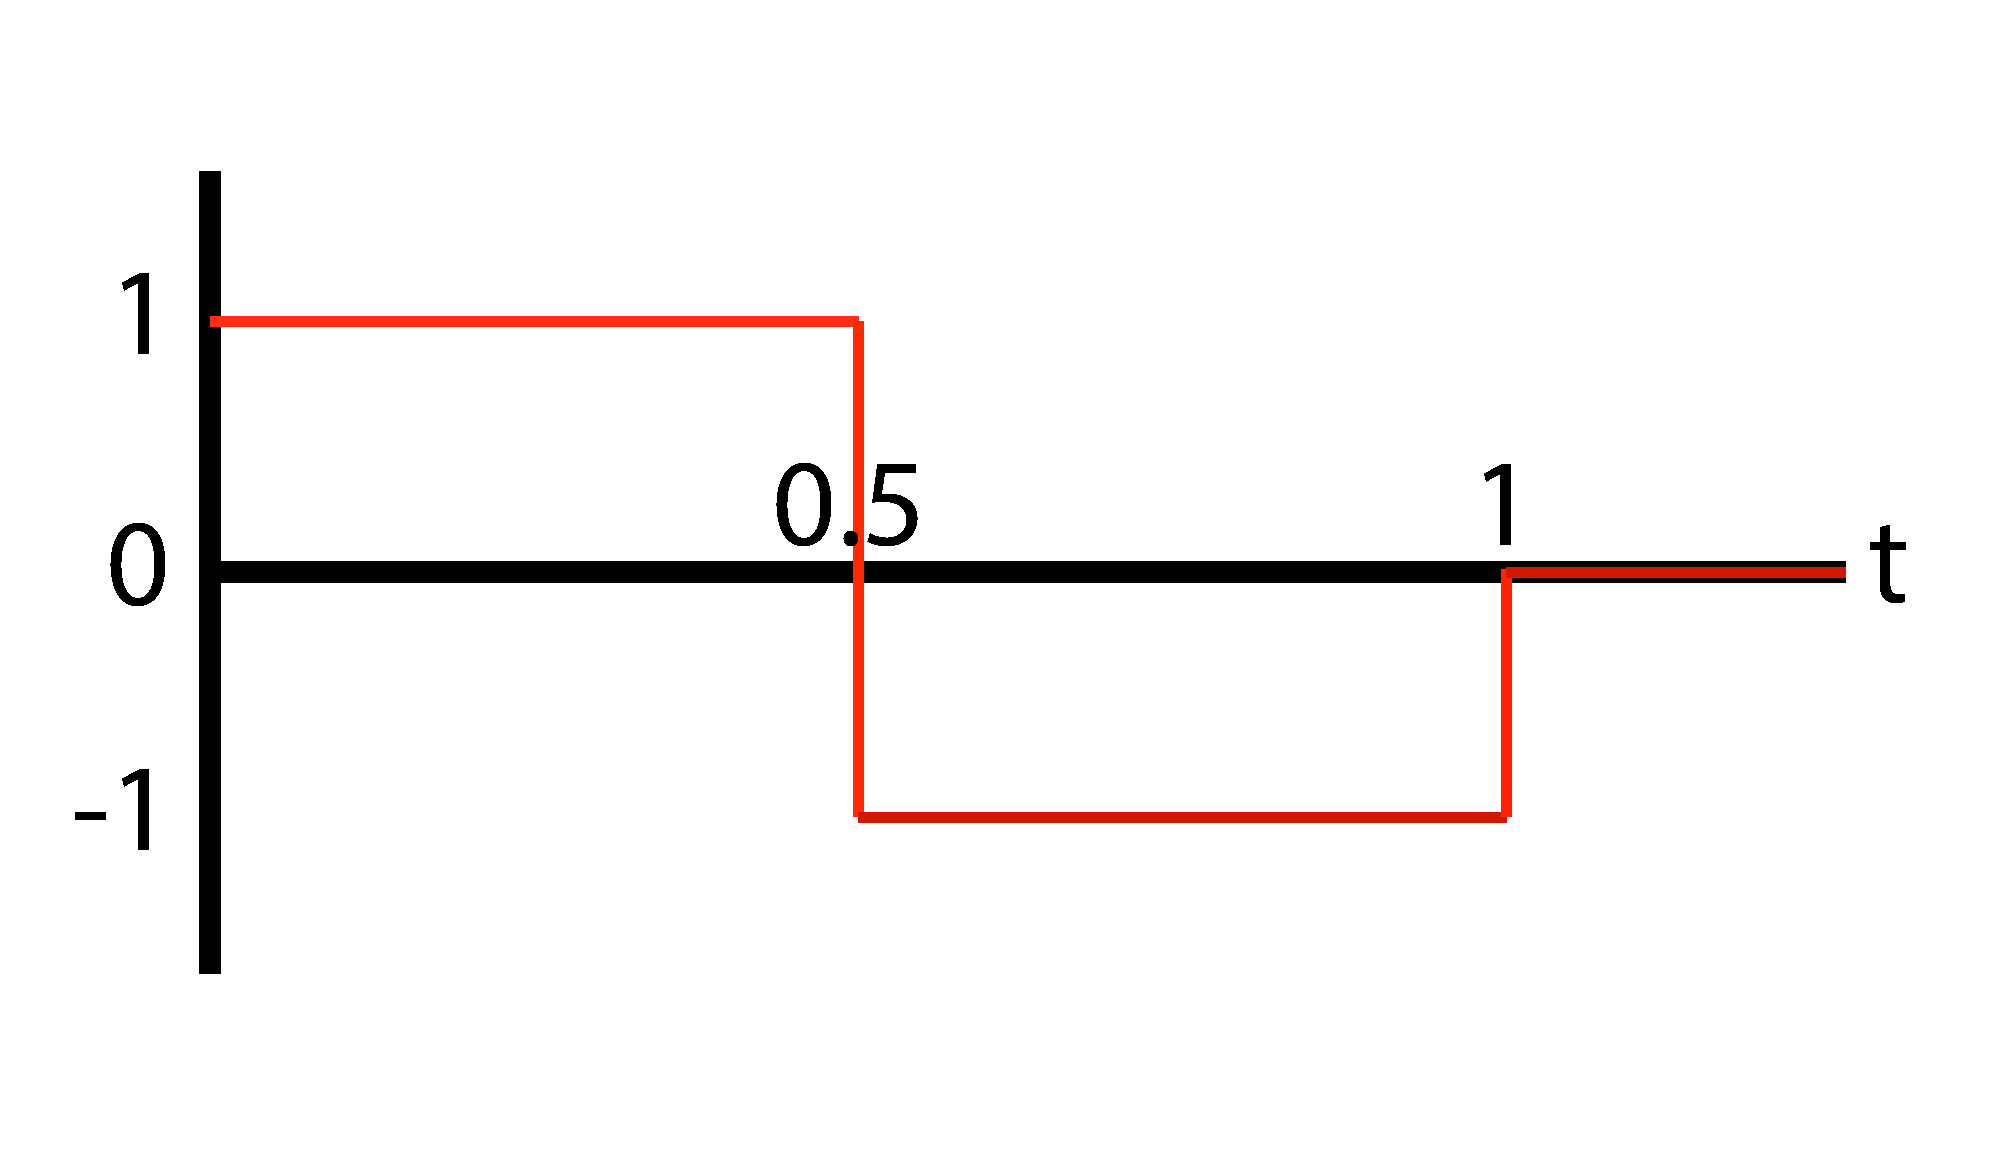
\includegraphics[height=3cm]{content/HaarWavelet.pdf}
	\end{minipage}	
	\begin{minipage}[c]{0.3\textwidth}
		\[
			\psi(t)=\begin{cases} 1 \quad 0 \leq t < \frac{1}{2}\\ -1 \quad \frac{1}{2} \leq t < 1  \end{cases}  
		\]
	\end{minipage}
\end{center}


\[  
	\psi_{m,n}(t)=\frac{1}{\sqrt{2^m}} \cdot \psi(\frac{t}{2^m} - n) = 2^{-m/2} \cdot \psi(2^{-m}t-n) 
	\qquad \qquad
	\psi_{m,n}  = \begin{cases} 
	\frac{1}{\sqrt{2^m}} \qquad 2^m n \leq t < 2^m(n+\frac{1}{2}) \\ 
	\frac{-1}{\sqrt{2^m}} \qquad 2^m(n+\frac{1}{2}) \leq t < 2^m(n+1)
	\end{cases}
\]

\[ 
	\nu_{m,n} = \langle \psi_{m,n} | f \rangle = \int_{-\infty}^{\infty}\psi_{m,n}(t) \cdot f(t) \,\mathrm{d}t
	\qquad \Longleftrightarrow \qquad
	f(t)=\sum_{m,n \in \mathbb{Z}} \nu_{m,n} \cdot \psi{m,n}
\]
	
\[  
	||f||^2 = \sum_{m,n \in \mathbb{Z}} |\nu_{m,n}|^2 \qquad \qquad ||f-f_N||^2 = ||f - \sum_{m,n \in \mathbb{Z}}^N \nu_{m,n} \cdot \psi_{m,n}||^2 = \sum_{k=N+1}^{\infty} |c_k|^2
\]

Haar-Transformation:
\begin{enumerate}
	\item Funktion abtasten bei $2^m(n+1/2)$ im Intervall $[a,b] \qquad u_{m,n}\approx \sqrt{2^m}f(2^m[n+1/2])$ 
	\item Die abgetastete Sequenz mit 0 auffüllen bis zu einer Zweierpotenz
	\item In jedem Schritt $u_{m+k+1}, \nu_{m+k+1}$ berechnen
\end{enumerate}

Schnelle Haar-Transformation:
\[  
	u_{m,n} = \dfrac{u_{m,2n}+u_{m,2n+1}}{\sqrt{2}} 
	\qquad \qquad
	\nu_{m,n} = \dfrac{u_{m,2n}-u_{m,2n+1}}{\sqrt{2}}
\]

Haar-Scalingfunction?
	\section{Fourier Reihe}

Orthonormal Basis der Fourierreihe:
\[  
	e_k=\{\frac{1}{\sqrt{2 \pi}}, \frac{\cos(x)}{\sqrt{2 \pi}}, \frac{\sin(x)}{\sqrt{2 \pi}}, \frac{\cos(2x)}{\sqrt{2 \pi}}, \frac{\sin(2x)}{\sqrt{2 \pi}}, ... \} 
	\qquad \qquad
	f(x) = \sum_{k=0}^{\infty}\overbrace{\langle e_k|f \rangle}^{c_k} e_k
\]

Fourierreihe-Koeffizient berechnen: (wobei $\omega = \frac{2\pi}{T}$)
\[ 	a_k = \frac{2}{T} \langle \cos(k\omega t)|f \rangle 
	\qquad \qquad 
	b_k = \frac{2}{T} \langle \sin(k\omega t)|f \rangle 
	\qquad \qquad
	c_k = \frac{1}{T} \langle \e^{k\omega t}|f \rangle = \frac{1}{T} \int_{t}^{t+T}f(s) \e^{-jk\omega s} \, \mathrm{d}s
\]

\subsection{Properties}
\[  
	f(t) = \sum_{k \in \mathbb{Z}} p_k \e^{jk\omega t} \qquad \qquad g(t) = \sum_{k \in \mathbb{Z}} q_k \e^{jk\omega t} \qquad \qquad h(t) = \sum_{k \in \mathbb{Z}} c_k \e^{jk\omega t} \qquad h \in L^2([0,T])
\]

Linearität:\[ h=af+bg \Longrightarrow c_k=ap_k+bq_k \]
Translation:\[ h(t)=f(t+s) \Longrightarrow c_k=p_k\cdot \e^{jk\omega s} \]
Produkt:\[ h=f\cdot g \Longrightarrow c_k=\sum_{l\in\mathbb{Z}}p_l\cdot q_{k-l} \]
Faltung:\[ h(t)=(f\ast g)(t)=\int_{\tau}^{\tau + T}f(s)g(t-s) \, \mathrm{d}s \Longrightarrow c_k=p_k \cdot q_k \]
Derivative:\[ h=f' \Longrightarrow c_k=jk\omega p_k \]

Wenn folgendes Theorem erfüllt ist hat $h$ n kontinuierliche Ableitungen:
\[ |c_k|<\dfrac{c}{(1+|k|)^{1+n+\epsilon}} \qquad n \in \mathbb{N} \quad k \in \mathbb{Z} \]



\newpage
\section{Fourier Transformation}

\begin{center}
	\begin{tabular}{c|c|c}
		& periodisch & nicht-periodisch \\
		\hline
		diskret & $h_t \leftrightarrow \hat{h}_k$ & $c_k$, $h_t$ \\
		\hline
		kontinuierlich & $f(t+T)$, $\hat{h}(\xi)=\hat{h}(\xi + 1)$ & $f(t)\Leftrightarrow \hat{f}(\xi)$
	\end{tabular}
\end{center}

\subsection{Linear and Time Invariant System (LTI)}
Sei $x$ eine $T$ periodische Funktion, dann ist $H$ ein LTI System wenn folgendes gilt (S ist die Shift-Matrix um $T$):
\[ 	H\cdot S = S\cdot H \qquad \qquad y=H\cdot x 
	\qquad \qquad 
	\text{Bsp. wenn T=3 ist: } \left( \begin{array}{ccc} x_2=x_{-1} \\ x_0 \\ x_1 \end{array} \right) = S_3 \cdot \left( \begin{array}{ccc} x_0 \\ x_1 \\ x_2 \end{array} \right) \quad
	S_3=
	\left( \begin{array}{ccc}
	0 & 0 & 1 \\
	1 & 0 & 0 \\
	0 & 1 & 0 
	\end{array} \right) 
\]


\subsection{Finite Fourier Transformation}
Die Eigenvektoren und Eigenwerte plus ein Faktor von einer LTI Matrix $H$ stellen die Finite Fourier Transformation dar: (wobei $\omega = \frac{2\pi}{T}$)\\

Eigenwerte: \[ \lambda_k = \sum_{t=0}^{T-1} h_t \e^{-jk\omega t} \]
Finite Fourier Transformation: \[ \hat{h}_k = c_T \cdot \lambda_k = c_T \cdot \sum_{t=0}^{T-1} h_t \e^{-jk\omega t} \]
Inverse Finite Fourier Transformation: \[ h_t = \frac{1}{c_T T} \cdot \sum_{k=0}^{T-1}\hat{h}_k \e^{+jk\omega t} \]
Wobei $c_T = \frac{1}{T}$. Mehr Symmetrie kann durch die Wahl von $c_T = \frac{1}{\sqrt{T}}$ erreicht werden. Dann gilt $||h||^2=||\hat{h}||^2$

%TODO abklären ob FFT noch eingefügt werden soll

\subsection{Fourierreihe, Laurentreihe, Z-Transformation}

Transferfunction: \[ H(z)=\sum h_k \cdot z^{-k} \qquad \text{(Z-Transformation)} \qquad \qquad z_k=\e^{jk\omega} \qquad z_k^0=z_k^T=1 \]
Frequenzgang: \[ \hat{h}(\xi) = H(\e^{2\pi j \xi})=\sum h_k \e^{-2\pi jk \xi} \qquad \text{Aplitudengang: } |\hat{h}(\xi)| \qquad \text{Phasengang: } \arg|\hat{h}(\xi)| \]

(Die DFT ist nur die inverse Fourierreihe mit Periode $T=1$ und einem Signum.)

\newpage
\subsection{Fouriertransformation on $\mathbf{L^2(\mathbb{R})}$}

Fouriertransform (FT): \[ \hat{f}(\xi) = \int_{-\infty}^{\infty}f(t) \e^{-j 2\pi \xi t} \, \mathrm{d}t \qquad \qquad \xi = \frac{k}{T} \text{ wobei } (T \rightarrow \infty) \]

Inverse Fouriertransform (IFT): \[ f(t) = \int_{-\infty}^{\infty}\hat{f}(\xi) \e^{+j 2\pi \xi t} \, \mathrm{d}\xi \]

Plancherel Identity: \[ ||f(t)||^2 = ||\hat{f}(\xi)||^2 \]

\subsubsection{Properties}
Linearität: \[ h = af + bg \FT \hat{h} = a\hat{f + b\hat{g}} \]
Translation: \[ h(t) = f(t+s) \FT \hat{h}(\xi) = \hat{f}(\xi) \cdot \e^{j2\pi\xi s} \]
Produkt: \[ h = f \cdot g \FT \hat{h} = (\hat{f}\ast\hat{g})(\xi) = \int \hat{f}(\xi) \hat{g}(\xi - s) \,\mathrm{d}s \]
Faltung: \[ h = (f\ast g)(t) \FT \hat{h} = \hat{f} \cdot \hat{g} \]
Derivative: \[ h = f' \FT \hat{h} = j2\pi\xi\cdot\hat{f}(\xi) \]
Scaling: \[ h(t) = f(at) \FT \hat{h}(\xi) = \frac{1}{|a|} \cdot \hat{f}(\frac{\xi}{a}) \]

\subsubsection{Unschärferelation}
Je mehr das Signal bei 0 konzentriert ist, desto kleiner ist die Varianz $\int\limits_{\mathbb{R}} t^2 \cdot |f(t)|^2 \,\mathrm{d}t$.\\
Die Aussage der Unschärferelation: Lokale Information wird von der FT verschmiert!
(Grosse Varianz: schlecht konzentriert, kleine Varianz: gut konzentriert)

\[  
	\int\limits_{-\infty}^\infty t^2 \cdot |f(t)|^2 \, \mathrm{d}t \cdot \int\limits_{-\infty}^\infty \xi^2 \cdot |f(\xi)|^2 \, \mathrm{d}\xi
	\geq \frac{1}{16 \pi^2} ||f||^2||\hat{f}||^2 \underbrace{= \frac{1}{16 \pi^2} ||f||^4}_{\text{ Plancherel}}
\]

Wenn $f(t)=C \cdot \mathrm{e}^{-kt^2}$ aufweist, kann das $=$ in der obigen Ungleichung erreicht werden. (Wird die Fouriertransformation ohne $2\pi$ im Exponent definiert, dann wird der Faktor $\frac{1}{16\pi^2}$ zu $\frac{1}{4}$)

%\subsubsection{Sampling, Undersampling, Aliasing}
%TODO: Abklären ob Samplingtheorem und Aliasing benötig wird?
	\newpage
	\section{Multiresolution Analysis (MRA)}

Skalierungsfunktion (Mother scaling function $\varphi(t)$): 
\[
	\varphi_{m,n}(t)=2^{-m/2} \cdot \varphi(2^{-m}\cdot t - n) = \frac{1}{\sqrt{2^{m}}} \cdot \varphi(2^{-m}\cdot t -n) = 2^{-m/2} \cdot \varphi(2^{-m}\cdot (t - 2^{m}\cdot n))
\]

Forderung an die Skalierungsfunktion:\\
(Aussage von 2-scaling: Eine Funktion wird um den Faktor 2 (in der Zeit) gestaucht. Durch verschieben, strecken bzw. stauchen (der Amplitude) und aufaddieren dieser skalierten Funktion, kann die  Ausgangsfunktion wieder dargestellt werden.)
\[
	\langle \varphi_{0,n}|\varphi_{0,n'} \rangle = \delta_{n,n'} =  \begin{cases} 1 \quad n=n'\\ 0 \quad sonst  \end{cases}  \qquad \text{orthonormality} 
\]
\[
	\varphi(t) = \sqrt{2} \sum_{k \in \mathbb{Z}} h_k \cdot \varphi(2t-k) = \sum_{k \in \mathbb{Z}} h_k \cdot \varphi_{-1,k}(t) \qquad \varphi_{m,n}=\sum_{k \in \mathbb{Z}} h_k \cdot \varphi_{m-1,2n+k} \qquad \text{2-scaling}  
\]
\[
	\varphi \text{ muss integrierbar sein und } \int_{-\infty}^{\infty}\varphi(t) \mathrm{d}t = 1  \qquad \text{mean one}  
\] 


Scale space (je weiter nach rechts (je kleiner m), desto grösser der Raum): 
\[
	...\subset V_{m+1} \subset V_{m} \subset V_{m-1} \subset ...
	\qquad \qquad
	V_m = \langle \varphi_{m,n}|n \in \mathbb{Z}  \rangle = \{ ...,\varphi_{m,-1},\varphi_{m,0}, \varphi_{m,1}, \varphi_{m,2},... \}
\]

Detail space (Detailinformation):
\[
	W_m = \langle \psi_{m,n} | n \in \mathbb{Z} \rangle
	\qquad \qquad
	V_{m-1} = V_m \oplus W_m
\]

Wavelet:
\[
	\psi_{m,n} = \sum_{k \in \mathbb{Z}} g_k \varphi_{m-1,2n+k} 
\]

Definition vom scale coefficient $u_{m,n}$ und dem detail coefficient $v_{m,n}$:
\[
	u_{m,n} = \langle \varphi_{m,n}|f \rangle
	\qquad \qquad
	v_{m,n} = \langle \psi_{m,n}|f \rangle
\]

Fast Wavelet Transform (Decomposition / Reconstruction):
\[
	\boxed{\begin{array}{ccccc}
		u_m & \xrightarrow{H'} & u_{m+1} & \xrightarrow{H'} & u_{m+2} \\
		& \searrow^{G'} & & \searrow^{G'} & \\
		& & v_{m+1} & & v_{m+2} \\
	\end{array}}
	\qquad \qquad \qquad \qquad
	\boxed{\begin{array}{ccccc}
		u_{m+2} & \xrightarrow{H} & u_{m+1} & \xrightarrow{H} & u_{m} \\
		& \nearrow_G & & \nearrow_G & \\
		v_{m+2}& & v_{m+1} & & \\
	\end{array}}
\]

\[  
	u_{m+1,n} = \sum_{k \in  \mathbb{Z}} h_{k-2n} u_{m,k} \quad v_{m+1,n} = \sum_{k \in  \mathbb{Z}} g_{k-2n} u_{m,k}
	\qquad \qquad
	u_{m,n} = \sum_{k \in  \mathbb{Z}} h_{n-2k} u_{m+1,k} + g_{n-2k} v_{m+1,k}
\]

\[
	H'(x)_n = \sum_{k \in  \mathbb{Z}} h_{k-2n} x_k
	\qquad \qquad \qquad \qquad
	H(x)_n = \sum_{k \in  \mathbb{Z}} h_{n-2k} x_k
\]

\[
	G'(x)_n = \sum_{k \in  \mathbb{Z}} g_{k-2n} x_k
	\qquad \qquad \qquad \qquad
	G(x)_n = \sum_{k \in  \mathbb{Z}} g_{n-2k} x_k
\]

	\newpage
	\section{Designing Wavelet Filters}

\subsection{Vanishing Moments}
 Wenn die Fouriertransformation $\hat{\psi}(\xi)$ eine Nullstelle der Ordnung $p$ an der Stelle $\xi = 0$ hat, dann sind die Ableitungen $\hat{\psi}^{(k)}(0)$ für $k=0,1,...,p-1$ gleich Null. Setzt man die Formel für die Fouriertransformation ein sieht man, dass das k-th Moment verschwindet!

\[ 
	\mu_k = \int_{-\infty}^{\infty} \psi(t) = t^k \, \mathrm{d}t
\]

Ein Wavelet sollte möglichst viel verschwindende Momente (vanishing moments) aufweisen, denn dann sind die Koeffizienten $\nu_{m,n} = 0$.

%TODO infos aus Anwenndungsteil hinzufügen + Weitere wichtige eigenschaften wie z.B. kurze Filter etc.


\section{Scaling Function From Filter Coefficients}
	\newpage
	\section{Anwendung}

\subsection{Datenkompression}

\subsubsection{Notation}
\begin{tabular}{ll}
$f$ & diskretes Signal\\
$B$ & Bit-Stream, repräsentiert eine Approximation von $f$ welches mit einer bestimmten Methode codiert wurde. \\
$\tilde{f}$ & Approximation von $f$ repräsentiert durch B, die komprimierte Version von $f$\\
$r$ & Kompressionsrate (zB.: $\dfrac{\text{Anzahl Bits in }f}{\text{Anzahl Bits in }B}$)\\
$\tilde{f}-f$ & Quantisierungsfehler, Quantisierungsrauschen, Verzerrung, Residual\\
\end{tabular}
\begin{tabular}{ll}
$\mathrm{MSE}(\tilde{f}) := \frac{1}{M \cdot N}\sum_{i=0}^{M-1}\sum_{k=0}^{N-1}\lvert \tilde{f}_{i,k}-f_{i,k} \rvert^2$ & Mean Squared Error vom komprimierten Bild\\
$\mathrm{PSNR}(\tilde{f}) := 10 \cdot \log_{10}(\frac{K^2}{\mathrm{MSE}(\tilde{f})})$ & Peak Signal to Noise Ratio, mit $K=\mathrm{max}\{\mathrm{max}(f)-\mathrm{min}(f)\}$ \\
 &  (Bei eine Graustufenbild mit der Farbtiefe 8 beträgt $K=255$)
\end{tabular}

\subsubsection{Vorgen für Datenkompression}
\[ 
	f \longrightarrow \boxed{\mathrm{Transformation}} \longrightarrow (c_k)_{k\in J} \longrightarrow \boxed{\mathrm{Quantisierung}} \longrightarrow (\tilde{c}_k)_{k \in J} \longrightarrow \boxed{\mathrm{Entroipy Coding}}\longrightarrow B 
\]

Ziel ist es das Signal $f$ in eine Basis zu Transformieren, bei der viel Koeffizienten 0 oder sehr klein werden. Bei der Quantisierung werden diese kleinen Koeffizienten auf 0 quantisiert. Diese Koeffizienten können durch eine effizientes Entropy Coding komprimiert abgespeichert werden.\\

Waveletkompression:
\begin{itemize}
	\item Analyse Wavelet: sollte einige verschwindende Momente haben
	\item Synthese Wavelet: die synthese Funktion sollte eine gute Regularität aufweisen
	\item alle Funktionen sollten Symmetrisch sein (gerade oder ungerade, "Lineare Phase")
	\item Orthogonalität
	\item kurze Filter für bessere Performance (Mehr verschwindende Momente und bessere Regularität erhöhen die Filterlänge)
\end{itemize}
Ein gutes Wavelet ist das bior4.4. Es ist biorthogonal, symmetrisch, hat 4 vanishing Moments, das Synthese Wavelet hat eine Regularität die grosser als 1.3 ist. Die resultierenden Filter weisen 7 bzw. 9 Filterkoeffizienten auf.


\subsubsection{Zwei-Dimensionale Wavelettransformation}

Die Operatoren $A_k$ berechnet den Approximationskoeffizient der Stufe $k$. Die Detailkoeffizienten der Stufe $k$ werden durch den Operator $D_k^j$ berechnet. Bei den Detailkoeffizienten wird unter horizontal $j=h$, vertikal $j=v$ und diagonalen $j=d$ Details unterschieden. (Horizontal=parallel zur x-Achse)

\begin{minipage}[c]{0.6\textwidth}
	\[  
		A_0f = A_mf+\sum_{1}^{k=m}(D_k^hf+D_k^vf+D_k^df)
	\]
	\[  
		A_kf(x,y)=\sum_{q\in\mathbb{Z}}\sum_{p\in \mathbb{Z}}u_{k;p,q}\Phi_{k;p,q}(x,y) = \sum_{q\in\mathbb{Z}}\sum_{p\in \mathbb{Z}}u_{k;p,q} \varphi_{k,q}(x) \varphi_{k,p}(y)
	\]
	\[  
		D_k^hf(x,y)=\sum_{q\in\mathbb{Z}}\sum_{p\in \mathbb{Z}}v_{k;p,q}^h\Psi_{k;p,q}^h(x,y) = \sum_{q\in\mathbb{Z}}\sum_{p\in \mathbb{Z}}v_{k;p,q}^h \varphi_{k,q}(x) \psi_{k,p}(y)
	\]
	\[  
		D_k^vf(x,y)=\sum_{q\in\mathbb{Z}}\sum_{p\in \mathbb{Z}}v_{k;p,q}^v\Psi_{k;p,q}^v(x,y) = \sum_{q\in\mathbb{Z}}\sum_{p\in \mathbb{Z}}v_{k;p,q}^v \psi_{k,q}(x) \varphi_{k,p}(y)
	\]
	\[  
		D_d^vf(x,y)=\sum_{q\in\mathbb{Z}}\sum_{p\in \mathbb{Z}}v_{k;p,q}^d\Psi_{k;p,q}^d(x,y) = \sum_{q\in\mathbb{Z}}\sum_{p\in \mathbb{Z}}v_{k;p,q}^d \psi_{k,q}(x) \psi_{k,p}(y)
	\]		
\end{minipage}
\begin{minipage}[c]{0.4\textwidth}
	\includegraphics[width=0.8\textwidth]{content/ZweiDimWaveletTransf.pdf}	
	\[ u_{k;q,p}=\langle f|\Phi_{k;q,p} \rangle = \iint_{\mathbb{R}^2} f \cdot \Phi_{k;q,p} \, \mathrm{d}x\mathrm{d}y \]
	\[ = \int_{-\infty}^{\infty} \int_{-\infty}^{\infty} f(x,y) \varphi_{k,q} \varphi_{k,p}(y) \, \mathrm{d}x\mathrm{d}y \]
\end{minipage}
\[
	v_{k;q,p}^h=\langle f|\Psi_{k;q,p}^h \rangle = \iint_{\mathbb{R}^2} f \cdot \Psi_{k;q,p}^h \, \mathrm{d}x\mathrm{d}y = \int_{-\infty}^{\infty} \int_{-\infty}^{\infty} f(x,y) \varphi_{k,q} \psi_{k,p}(y) \, \mathrm{d}x\mathrm{d}y \qquad \text{etc.}
\]

Die Filterkoeffizienten werden aber mit der Oben abgebildeten Filterbank berechnet.


\subsection{Denoising}

\subsubsection{Notation}

\begin{tabular}{ll}
	$f$ & gemessenes Signal (Sequenz von Samples $f_1, f_2,...$), $f=f^\# + f^R$ \\
	$f^\#$ & richtiges Signal (unbekannt) \\
	$f^R$ & Rauschen (unbekannt, stochastisch) \\
	$\tilde{f}$ & Schätzung des richtigen Signals \\
	$\mathrm{MSE}(\tilde{f}) := \frac{1}{N}\sum_{k=0}^{N-1}|\tilde{f}_k - f_k^{\#}|^2$ & Mean Squard Error \\
\end{tabular}

Signal to Noise Ratio (SNR):
\[
	\mathrm{SNR}(\tilde{f}):=10\cdot \log_{10} \left(\frac{1}{N}\sum_{k=0}^{N-1} |f_k^{\#}|^2 / \mathrm{MSE}\right) = \left(\sum_{k=0}^{N-1} |f_k^{\#}|^2 / \sum_{k=0}^{N-1}|\tilde{f}_k - f_k^{\#}|^2\right)
\]

\subsubsection{Vorgehen für Denoising}
\[ 
	f \longrightarrow \boxed{\mathrm{Transformation}} \longrightarrow (v_{m,n}) \longrightarrow \boxed{\mathrm{Thresholding}} \longrightarrow (\tilde{v}_{m,n}) \longrightarrow \boxed{\mathrm{Reconstruction}}\longrightarrow \tilde{f} 
\]

Mit der Annahme, dass die grössten Koeffizienten für die Signalbeschreibung ausreichend sind, kann davon ausgegangen werden das das Rauschen in vielen kleinen Koeffizienten enthalten ist. Ist dies der Fall wird durch Thresholding das Rauschen eliminiert und das wahre Signal nicht gross beeinträchtigt.

Der Vorteil beim Denoising mit Wavelet ist, zum Ersten dass im Zeit- und Frequenzbereich gleichzeitig gearbeitet wird und zum Zweiten dass Signale, die ihre Eigenschaften mit der Zeit ändern, einfach behandelt werden können (zB: Sprünge). 

\vspace{0.5cm}

\begin{minipage}[c]{0.5\textwidth}
	Hard-Thresholding mit der Grenze $\tau$:
	\[ \tilde{v}_{m,n} := \begin{cases} 0 \qquad |v_{m,n}| \leq \tau \\ v_{m,n} \qquad |v_{m,n}| > \tau \end{cases} \]
\end{minipage}
\begin{minipage}[c]{0.5\textwidth}
	Soft-Thresholding (shrinkage) mit Grenze $\tau$:
	\[ \tilde{v}_{m,n} := \begin{cases} 0 \qquad |v_{m,n}| \leq \tau \\ \mathrm{sign}(v_{m,n}) \cdot (|v_{m,n}-\tau|) \qquad |v_{m,n}| > \tau \end{cases} \]
\end{minipage}

Gute Resultate werden unter den folgenden Voraussetzungen erreicht:
\begin{itemize}
	\item das Signal kann vom Wavelet gut komprimiert werden
	\item das Rauschen kann nicht komprimiert werden
	\item SNR($f$) ist genügend gross
\end{itemize}


Wahl von $\tau$, wobei die Schätzung für $sigma_m$ nur für Rauschen gilt, das gaussverteilte Waveletkoeffizienten aufweist:

\begin{minipage}[c]{0.5\textwidth}
\[
	\tau_m \approx K \cdot \sqrt{2 \cdot \ln(N)} \cdot \sigma_m  
\]
\[
	\sigma_m \approx \dfrac{\mathrm{median}(|v_{m,n}| \, | n \in  \mathbb{Z})}{0.6745} 
\]
\end{minipage}
\begin{minipage}[c]{0.5\textwidth}
$K \in [0.2,1.6]$\\
$N$: Anzahl Samples des Signals $f$\\
median: Ein Wert $m$ ist der Median von einer Menge von Werten wenn die Hälfte aller Werte $\leq m$ und die andere Hälfte $\geq m$ ist.
\end{minipage}

\begin{itemize}
	\item White-Noise: Gleiche Grenze $\tau = \tau_1$ in allen Scales ($m=1$ Finest Scale)
	\item Colored-Noise: Die Grenue $\tau$ wird an jede Scale $m$ angepasst.
\end{itemize}


\subsubsection{Stationary  Wavelet Transformation (SWT)}
Die Stationäre Wavelet Transformation ist Translation-Invariant (shift-invariant). Die normale Wavelet Transformation ist nicht Translation-Invariant, dies kommt vom downsamplen. Wenn die Anzahl Scales $J$ ist, kann das Signal $f$ $2^J$ mal verzögert werden, bis wieder das gleiche entrauschte Signal berechnet wird. Aus diesem Grund berechnet die SWT  $2^J$ mal die DWT von verzögerten Signal $f$. Bei alle $2^J$ berechneten DWT wird die Verzögerung rückgängig gemacht und gemittelt. Das dabei entstehende Signal ist die SWT von $f$. 

\[ 
	\tilde{f}^{tr.inv} := \dfrac{1}{2^J} \sum_{k=0}^{2^J-1}T_k \left( \tilde{T}_k(f) \right) 
	\qquad \qquad
	T_k \text{: delay um $k$-Sample} \qquad \qquad J\text{: Anzahl Scales (Stages, Level)}
\]

Um $\tilde{f}^{tr.inv}$ zu berechnen, steigt die Berechnungszeit um Faktor $2^J$ an. Es gibt effizientere Methoden, bei denen der Aufwand auf Faktor $J$ reduziert werden kann.

Die SWT lässt das Downsamplen weg, upsampled statt dessen die Filter! Bei der SWT gibt es redundante Informationen über $f$, was schlecht für Kompressionen aber gut für Denoising (smoothing artifacts caused by thresholding) ist.

\begin{minipage}[l]{0.5\textwidth}
	Die dazugehörige Filterbank: \\
	$A_m$ beschreibt den um Faktor 2 upgesampleten Filter $A$ (mit $2^m -1$ Nullen zwischen zwei Filterkoeffizienten eingefügt $(...,a0,0,...,0,a1,0,...,0,a2,0,...)$ )
\end{minipage}
\begin{minipage}[r]{0.5\textwidth}
	\flushright
	\includegraphics[width=.9\textwidth]{content/swtFilterbank.pdf}
	\[ \tilde{f}^{tr.inv.}=\mathrm{ISWT}(\mathrm{shrink}(\mathrm{SWT}(f)) \]
\end{minipage}


\subsubsection{Abhängigkeit vom MSE und dem Threshold}
\[ MSE(\tilde{f}) = \frac{1}{N} \sum |v_{m,n}|^2 = \frac{1}{N}\left(\underbrace{\sum_{|v_{m,n}| < \tau}|v_{m,n}|^2}_{Rauschenergie} + \underbrace{\sum_{|v_{m,n}| \geq \tau}|v_{m,n}|^2}_{Signalenergie}\right) \]


\subsection{Feature Detection and Extraction}

Feature eines Signals oder eines Bildes ist ein bestimmter Teil Information darin. In 1 Dimension sind dies Peaks, Sprünge oder irgend welche Muster (pattern). Bei Bilder handelt es sich meist um Kanten, Ränder und Ecken.

Feature Detection meint die Lokalisierung der Gebiete wo das Feature auftritt.

FRR: false rejection rate, die W'keit das der Detektor ein Auftretendes Feature übersieht\\
FAR: false acceptance rate, die W'keit das der Detektor ein Feature detektiert das keins ist

\subsubsection{Smooting and Differentiation}
\begin{minipage}[r]{0.5\textwidth}
Smoothing Kernal: $\Theta$\\
Skalierter Smoothing Kernal: $\Theta(\frac{\tau - t}{s})$\\
Smoothed Function: $f_s(t) = \int f(\tau) \cdot \Theta(\frac{\tau - t}{s}) \, \mathrm{d}\tau$\\
Ableitung der Smoothed Function: 
\end{minipage}
\begin{minipage}[r]{0.5\textwidth}
	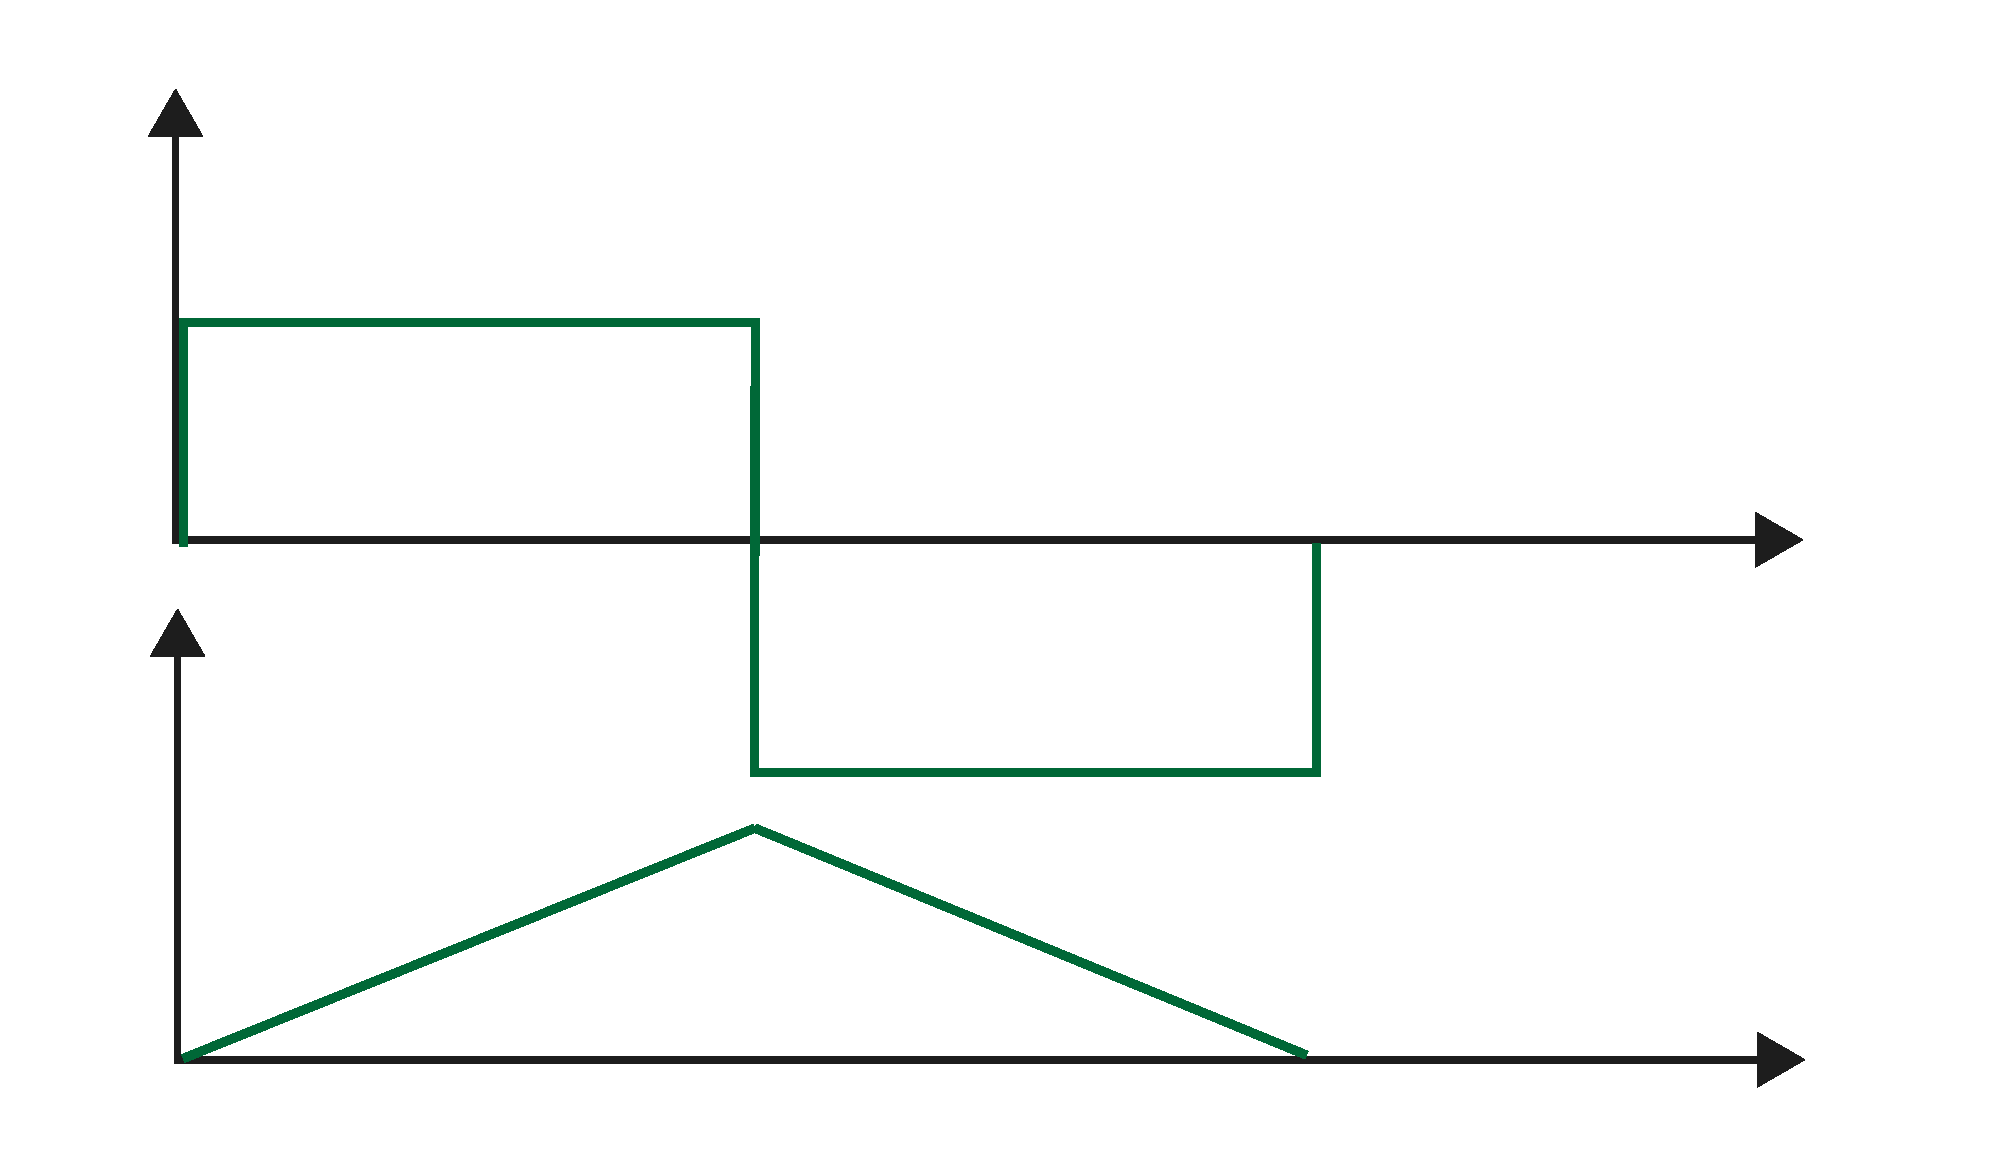
\includegraphics[width=0.4\textwidth]{content/SmoothingFunction.pdf}
	
	\vspace{-2.2cm}
	
	\flushright
	Abgeleiteter Smoothing Kernal
	
	\vspace{.4cm}
	
	Smoothing Kernal	
\end{minipage}

\[ \frac{\mathrm{d}}{\mathrm{d}t}f_s(t) = \int\limits_{-\infty}^{\infty} f(\tau) \cdot \frac{\mathrm{d}}{\mathrm{d}t}\Theta(\frac{\tau - t}{s}) \, \mathrm{d}\tau = -\frac{1}{s} \int\limits_{-\infty}^{\infty} f(\tau) \cdot \Theta'(\frac{\tau - t}{s}) \, \mathrm{d}\tau \]

Wavelet das integriert ein Smoothing Kernal ergibt: Haar-Wavelet ("Abgeleiteter Smoothing Kernal")\\
Daraus Folgt das die DWT oder SWT (besser) für die Approximation der Ableitung der Smoothed Function verwendet werden kann. Wird die SWT verwendet, dann kennt man die Ableitung der Funktion an allen Punkten.
\[ 
	\frac{\mathrm{d}f}{\mathrm{d}t} \approx C(m) \cdot v_{m,n}
	\qquad \qquad
	v_{m,n} =  \int\limits_{-\infty}^{\infty} f(\tau) \psi_{m,n}(\tau) \, \mathrm{d}\tau 
\]
Das Integral vom Smoothing Kernal muss 1 ergeben, damit das Mittel von $f$ gleich bleibt: 
\[ \int \underbrace{\int C(m) \psi_{m,n}(\tau) \,\mathrm{d}\tau}_{\Theta} \,\mathrm{d}t = 1 \]


\subsection{Matlab}

	
	%Anhang
	\newpage
	\appendix
	\section{Lineare Algebra}

\subsection{Vektoren}

\subsubsection{Betrag von Vektoren}
\[ 
	|\vec{a}| = \sqrt{\vec{a} \cdot \vec{a}} = ||\vec{a}|| =\sqrt{a_1^2 + a_2^2 + \ldots + a_n^2}
\]

	
\subsubsection{Skalarprodukt}
\[ 
	\vec{a} \cdot \vec{b} = a_1 \cdot b_1 + a_2 \cdot b_2 + \ldots +a_n \cdot b_n = |\vec{a}| \cdot |\vec{b}| \cdot \cos(\varphi)
\]
			
Projektion $\vec{p}$ vom Vektor $\vec{a}$ auf den Einheitsvektor $\vec{e}$ (wobei $|\vec{e}|=1$): \hspace{1cm} $\vec{p}=(\vec{a} \cdot \vec{e}) \cdot \vec{e}$


\subsubsection{Vektorprodukt}
\[
	\vec{a} \times \vec{b} = 
	\begin{pmatrix}a_1\\a_2\\a_3 \end{pmatrix} \times 
	\begin{pmatrix}b_1\\b_2\\b_3 \end{pmatrix} = 
	\begin{pmatrix}
	a_2 b_3 - a_3 b_2 \\ a_3 b_1 -  a_1 b_3 \\ a_1 b_2 - a_2 b_1 
	\end{pmatrix} \quad \quad 
	|\vec{a} \times \vec{b}|=|\vec{a}| \cdot |\vec{b}| \cdot
	\sin(\varphi)
\]

Der Betrag von $|\vec{a} \times \vec{b}|$ entspricht der Fläche des
Parallelogramms das von $\vec{a}$ und $\vec{b}$ aufgespannt wird. Der Vektor  $\vec{a} \times \vec{b}$ steht senkrecht auf den Vektoren $\vec{a}$ und $\vec{b}$!

	
\subsection{Matrizen}

\subsubsection{Matrizenprodukt}
Matrizenprodukt (Skalarprodukt) einer Matrix A und einer Matrix B ergiebt eine
Matrix C, deren Elemente die Skalarprodukte der Zeilenvektoren von A mit den
Spaltenvektoren von B sind.

\[
	\begin{pmatrix}
	a_{11} & \ldots & a_{1n} \\
	\vdots & A & \vdots \\
	a_{n1} & \ldots & a_{nn}
	\end{pmatrix} \cdot \begin{pmatrix} 
	b_{11} & \ldots & b_{1n} \\
	\vdots & B & \vdots \\
	b_{n1} & \ldots & b_{nn}
	\end{pmatrix} = \begin{pmatrix}
	\sum\limits_{i=1}^n a_{1i}b_{i1} & \ldots & \sum\limits_{i=1}^n a_{1i}b_{in}
	\\ \vdots & C & \vdots \\
	\sum\limits_{i=1}^n a_{ni}b_{i1} & \ldots & \sum\limits_{i=1}^n a_{ni}b_{in}
	\end{pmatrix}
\]


\subsubsection{Rang}
Der Rang einer Matrix gibt an, wie viele Zeilen linear unabhängig sind.


\subsubsection{Spur}
Die Spur einer Matrix $A$ wird durch die Summe der Diagonalelemente berechnet.

\[
	\mathrm{Spur}(A)=\mathrm{tr}(A)=\sum\limits_{i=1}^n a_{ii}
\]

Rechenregeln:\\
- $\mathrm{Spur}(A)=\mathrm{Spur}(A^t)$\\
- $\mathrm{Spur}(AB)=\mathrm{Spur}(BA)$\\
- $\mathrm{Spur}(ABC)=\mathrm{Spur}(CBA)=\mathrm{Spur}(BCA)$\\

Anwendung: $\mathrm{Spur}(A)=1+2 \cos(\alpha)$

\subsubsection{Transponierte Matrix}
Transponierte Matrix $A^t$ heisst alle Spalten und Zeilen
der Matrix $A$ vertauschen.

\[
	A=  
	\begin{pmatrix} 
		a_{11} & a_{12} & \cdots & a_{1n} \\
		a_{21} & a_{22} & \cdots & a_{2n} \\
		\vdots & \vdots & \ddots & \vdots \\
		a_{m1} & a_{m2} & \cdots & a_{mn} \\
	\end{pmatrix}
	\qquad \qquad 
	A^{\mathrm{T}} = 
	\begin{pmatrix} 
		a_{11} & a_{21} & \cdots & a_{m1} \\
		a_{12} & a_{22} & \cdots & a_{2n} \\
		\vdots & \vdots & \ddots & \vdots \\
		a_{1n} & a_{2n} & \cdots & a_{mn} \\
	\end{pmatrix}
\]

Rechenregeln:\\
- $(A+B)^t=A^t+B^t$\\
- $(A \cdot B)^t=A^t \cdot B^t$


\subsubsection{Orthogonale Matrix}
Eigenschaften:\\
- Quadratisch\\
- Zeilenvektoren sind orthonormal, Spaltenvektoren sind orthonormal\\
- Multiplikation von 2 orthogonalen Matrizen gibt eine orthogonale
Matrix\\
- $A^t=A^{-1}$ und $A^t \cdot A = I$(Einheitsmatrix)\\
- Determinante hat immer Betrag $1$\\
- $\det(O)=+1$: die orthogonale Matrix $O$ enthält alle Drehungen\\
- $\det(O)=-1$: die orthogonale Matrix $O$ enthält alle Drehspiegelungen 


\subsubsection{Determinante (Quadratische Matrizen)}
\textbf{Berechnung:} \\
Die Determinante ist das Produkt der Pivoelemente $p$ (mit
Gauss ermittelbar).  $\det \begin{pmatrix}p_1 & \ldots & \ast \\
\vdots & p_i & \vdots \\ \ast & \ldots & p_n \end{pmatrix} =
\sum\limits_{i=1}^{n}p_i$\\

2D Matrix (Fisch): \hspace{1cm} $\det \begin{pmatrix}a & b \\ c
& d \end{pmatrix} = a d - b c$\\

\textbf{Rechenregeln:}\\
- $\det(A \cdot B) = \det(A) \cdot \det(B)$\\
- $\det(A^{-1})=\det(A)^{-1}=\frac{1}{\det(A)}$\\
- $\det(A^t)=\det(A)$ wenn $A$ Quadratische \\

\textbf{Merksätze:}\\
- Matrix $A$ linear abhängig $\Rightarrow \det(A)=0$\\
- Vertauschen von 2 Zeilen $\Rightarrow (-1)\cdot \det(A)$\\
- Determinante einer 2D Matrix entspricht der Fläche des aufgespannten
Parallelogramm\\
- Determinante einer 3D Matrix entspricht dem Volumen des aufgespannten
Parallelepipeds\\
- Determinante einer orthagonalen Matrix hat immer Betrag $1$

\subsubsection{Cramersche Regel}
Ausgangslage: $\qquad A \cdot x = b \qquad \det(A)\neq 0$\\
Lösung $x_i$:
\[
	x_i=\frac{\det(A_i)}{\det(A)} \qquad \qquad A_i:\text{ $i$-te Spalte von $A$  durch rechte Seite  $b$ ersetzen!}
\]


\subsection{Eigenvetoren und Eigenwerte}
Ein Eigenvektor $v$ einer Abbildung $A$ (Matrix) ist ein vom Nullvektor
verschiedener Vektor, dessen Richtung durch die Abbildung nicht verändert wird. Der Vektor wird nur
gestreckt oder gestaucht. Dieser Faktor wird Eigenwert $\lambda$ genannt.
\[
	A v = \lambda v \quad \Leftrightarrow \quad (A-\lambda I)v=0
\]

\textbf{Charakteristisches Polynom:}\\
\[
	\chi_A(\lambda)=\det(A-\lambda I)
\]

\textbf{Eigenwerte:}\\
Die Nullstelle (da $A-\lambda I$ Singulär) des charakteristischen Polynom sind
die Eigenwerte. 
\[
	\chi_A(\lambda)=\det(A-\lambda I)=0
\]

\textbf{Eigenvektoren:}\\
Um die Eigenvektoren zu erhalten muss das folgende Gleichungssystem für jeden
Eigenwert gelöst werden.
\[ 
	(A-\lambda I)v=0 \qquad \qquad (v \text{ auf länge 1 normieren})
\]

\subsection{Spezielle Matrizen}
Einheitsmatrix: 
$I= \begin{pmatrix} 
1 & 0 & 0 \\
0 & 1 & 0 \\
0 & 0 & 1
\end{pmatrix}$

\vspace{0.5cm}

Drehmatrizen:
$\quad$
X-Achse
$\begin{pmatrix} 
	1 & 0 & 0 \\
	0 & \cos(\alpha) & -\sin(\alpha) \\
	0 & \sin(\alpha) & \cos(\alpha)
\end{pmatrix}$
$\quad$
Y-Achse
$\begin{pmatrix} 
	\cos(\alpha) & 0 & \sin(\alpha) \\
	0 & 1 & 0 \\
	-\sin(\alpha) & 0 & \cos(\alpha)
\end{pmatrix}$
$\quad$
Z-Achse
$\begin{pmatrix} 
	\cos(\alpha) & -\sin(\alpha) & 0 \\
	\sin(\alpha) & \cos(\alpha) & 0 \\
	0 & 0 & 1
\end{pmatrix}$

	\section{Faltung}
Faltung:
\begin{equation}
  \nonumber
  y(t) = f(t) \ast g(t) = \int\limits_{-\infty}^{\infty}f(u) \cdot g(t-u) du
\end{equation}

Periodisch:
\begin{equation}
  \nonumber
  y(t) = f(t) \ast g(t) = \frac{1}{T}\int\limits_{a}^{a + T}f(u) \cdot g(t-u) du
\end{equation}

Diskret:
\begin{equation}
  \nonumber
  y(i)=f(i) \ast g(i)=\sum\limits_{k=-\infty}^{\infty}f(k)\cdot g(i-k)
\end{equation}

\begin{tabular}{p{9cm}p{9cm}}
  Interpretation: & Geltende Rechengesetze:\\
  \begin{enumerate}
    \item $g(t)$ an der Y-Achse Spiegeln
	  \item Verschiebung um $t$ nach rechts
	  \item Durch Multiplikation der beiden Signale entstehende Fläche berechnen
  \end{enumerate}
&
  \begin{itemize}
    \item Kommutativ (Vertauschen) $g \ast f = f \ast g $
	  \item Distributiv (Ausklammern, Ausmultiplizieren) $g \ast(f \ast h) = g \ast f \ast h$
	  \item Assoziativ (Reihenfolge von Klammern) $g \ast(f \ast h) = (g \ast f) \ast h$
	  \item Faltung mit Dirac $\delta(t-t_0) \ast f(t) = f(t-t_0)$
  \end{itemize}
\end{tabular}
	
	
	

	\newpage
	\section{Fourierreihe}
Komplex:
\begin{equation}
\nonumber
\boxed{f(t) = \sum\limits_{k = -\infty}^{\infty} c_k \cdot e^{j k  	\omega_f t}}= \sum\limits_{k = 0}^{\infty} \left(c_k \cdot e^{j k \omega_f t} + \overline{c_k} \cdot e^{-j k \omega_f t}\right) \quad  \boxed{c_k=\overline{c_{-k}}=\frac{1}{T}\int_0^T{f(t)\cdot 	e^{-jk\omega_f t}dt}}
\end{equation}
	
\vspace{0.5cm}

Reell:
\[
\boxed{f(t) = \frac{a_0}{2} + \sum\limits_{k=1}^{\infty} \left[a_k \cos(k \omega_f t) + b_k \sin(k \omega_f t)\right]}=\frac{A_0}{2} + \sum\limits_{k=1}^{\infty} A_k \cos(k\omega_f t + \varphi_k) \quad k\in
  	\mathbb{Z}
\]	
	
\[\boxed{a_0 =
	\frac{2}{T}\int\limits_0^{T} f(t)dt, \quad a_k = \frac{2}{T}\int\limits_0^{T} f(t)\cos(k \omega_f t) dt, \quad b_k =
	\frac{2}{T}\int\limits_0^{T} f(t)\sin(k \omega_f t) dt} \quad
	\omega_f=\frac{2 \pi}{T}=2 \pi f
\]
	
\vspace{0.5cm}

$a_0$, $c_0$, $A_0$ sind \textit{Konstanten}, $\omega_f$ ist die \textit{Grundkreisfrequenz}, $a_k$ und $b_k$ sind die \textit{reellen Koeffizienten}, 
$c_k$ ist der \textit{komplexe Koeffizient}, $A_k$ ist die \textit{Amplitude} und $\varphi_k$ ist die \textit{Phase}.

\begin{tabular}{p{9cm}p{9cm}}
  $a_k = c_k + \bar{c_k} = 2 \text{Re}(c_k) = A_k \cos(\varphi_k)$ &
  $b_k = j(c_k + \bar{c_k}) = -2 \text{Im}(c_k) = -A_k \sin(\varphi_k)$ \\
  $c_k = \frac{a_k-jb_k}{2} = \frac{A_k}{2} e^{j\varphi_k}$ &
  $c_{-k} = \overline{c_k} = \frac{a_k+jb_k}{2} = \frac{A_k}{2} e^{-j\varphi_k}$ \\
  $A_k = 2|c_k| = \sqrt{a_k^2+b_k^2}$
\end{tabular}

\vspace{0.5cm}

Berechnung von $\varphi_k$ aus $a_k$ und $b_k$:\\
\begin{tabular}{p{2.5cm}p{3.5cm}p{2cm}p{2.5cm}p{3.5cm}}
	$a_k> 0:$ & $\varphi_k = -\arctan(\frac{b_k}{a_k})$ & &
	$a_k<0:$ &	$\varphi_k = -\arctan(\frac{b_k}{a_k}) + \pi$\\
	%\hline
	$a_k = 0; b_k > 0:$ &	$\varphi_k = -\frac{\pi}{2}$ & &
	$a_k = 0; b_k < 0:$ &	$\varphi_k = \frac{\pi}{2}$\\
	%\hline
	$a_k = b_k = 0:$ &	$\varphi_k = \text{nicht definiert}$ & & & $\varphi_k =
	arg(c_k)$
\end{tabular}

\subsection{Symmetrie}
\begin{tabular}{|p{4.3cm}|p{4.3cm}|p{4.3cm}|p{4.3cm}|}
  \hline
 	\textbf{gerade Funktion} & \textbf{ungerade Funktion} &
 	\textbf{Halbperiode 1} & \textbf{Halbperiode 2}\\
 	%\hline
 	\includegraphics[width=3cm]{content/appendix/geradeFunktion.png}&
 	\includegraphics[width=3cm]{content/appendix/ungeradeFunktion.png}&   
  \includegraphics[width=3cm]{content/appendix/halbperiode1.png}&   
  \includegraphics[width=3cm]{content/appendix/halbperiode2.png}\\
	& & & \\			
	$f(-t)=f(t)$ & $f(-t)=-f(t)$ & $f(t)=f(t+\pi)$ & $f(t)=-f(t+\pi)$\\
	$b_k=0$ & $a_k=0$ & $a_{2k+1}=0$ & $a_{2k}=0$\\
	$a_k = \frac{4}{T} \int\limits_0^{\frac{T}{2}} f(t) \cdot \cos(k \omega_f
	t) dt$ &
	$b_k =  \frac{4}{T} \int\limits_0^{\frac{T}{2}} f(t) \cdot
  \sin(k \omega_f t) dt$ &
	$b_{2k+1}=0$ & $b_{2k}=0$\\
	\hline
\end{tabular} 
    
     	
\subsection{Spektren}

\begin{tabular}{p{0.3\textwidth}p{0.3\textwidth}p{0.3\textwidth}}
	Kosinus- Sinusamplitudenspek. & 
	Einseitiges Ampl.-/ Phasenspek. &
	Zweiseitiges Ampl.-/ Phasenspek. \\
	\includegraphics[width=5cm]{content/appendix/cosSinSpectr.png} &
	\includegraphics[width=5cm]{content/appendix/EinseitigSpectr.png} &
	\includegraphics[width=5cm]{content/appendix/ZweiseitigSpectr.png}
\end{tabular}

Das einseitige und zweiseitige Spektrum unterscheiden sich nur im
Amplitudendiagramm. Das Phasendiagramm für positive $k$ ist identisch. Die
Amplitudenwerte sind hälftig auf die pos. und neg. $k$ verteilt.

\subsection{Rechenregeln}
\begin{tabular}{p{0.25\textwidth}p{0.25\textwidth}p{0.25\textwidth}p{0.25\textwidth}}
  Ableiten & $\frac{\text{d}}{\text{d}t}\sum c_n \e^{j\omega_0 n t}=\sum c_n' \e^{j \omega_0 n t}$ & $c_n'=j\omega_0 n c_n$ & $\omega_0 = \frac{2 \pi}{T}$ \\
  Integrieren & $\int \sum c_n \e^{j\omega_0 n t} = \sum \tilde{c_{n}} \e^{j\omega_0 n t}$ & $\tilde{c_n}=\frac{1}{j\omega_0 n}c_n$ & $n\neq 0$ \\
  Verschieben & $s(t) = \sum c_n \e^{j\omega_0 n t}$ & $s(t-\tau)=\sum c_{n\tau}\e^{j\omega_0 n t}$ & $c_{n\tau}=c_n \e^{-j\omega_0 n \tau}$
\end{tabular}

	\section{Fourier Transformation}
\[
\boxed{f(t) =  \frac{1}{2\pi}\int\limits_{-\infty}^{\infty}
F(\omega)e^{j\omega t}d\omega}=\frac{1}{2
\pi}\int\limits_{-\infty}^{\infty}(R(\omega) \cos(\omega t) + X(\omega)
\sin(\omega t))d\omega + \frac{j}{2 \pi}\int \limits_{-
\infty}^{\infty}(R(\omega) \sin(\omega t)- X(\omega) \cos(\omega t))d\omega
\]

\[	
\boxed{F(\omega) = \int\limits_{-\infty}^{\infty} f(t)e^{-j\omega t}dt}
= R(\omega) - j X(\omega) \quad R(\omega) = \int\limits_{-\infty}^{\infty}
f(t)\cos(\omega t)dt \quad \mbox{ und } \quad X(\omega)=
\int\limits_{-\infty}^{\infty}f(t)\sin(\omega t)dt 
\]

\newpage	
\subsection{Eigenschaften}
Fourierintegral existiert wenn  $\int\limits_{-\infty}^{\infty}|f(t)| dt < \infty$\\

\renewcommand{\arraystretch}{2}

\begin{tabular}{|p{8cm}|l c l|}
  \hline
 	Linearität & 
 	$\alpha\cdot f(t) + \beta\cdot g(t)$ & $\FT$ & $\alpha\cdot F(\omega) + \beta\cdot G(\omega)$\\
 	\hline
  Zeitumkehrung (Spiegelung an der Y-Achse)&
  $f(-t)$ & $\FT$ & $F(-\omega) = F^*(\omega)$ \\
	\hline        	
	Ähnlichkeit &
	$f(\alpha t)$ & $\FT$ & $\frac{1}{|\alpha|}F \left (\frac{\omega}{\alpha} \right) \quad\alpha \in\mathbb{R}\setminus \{0\}$\\
	\hline
	Verschiebung im	Zeitbereich &
	$f(t\pm t_0)$ & $\FT$ & $F(\omega)e^{\pm j\omega t_0}$\\
	\hline
  Verschiebung im Frequenzbereich &
	$f(t)e^{\pm j\omega_0 t}$ & $\FT$ & $F(\omega\mp\omega_0)$\\
	\hline
	Ableitung im Zeitbereich &
	$\frac{\partial^n f(t)}{\partial t^n}$ & $\FT$ & $(j\omega)^n F(\omega)$\\
	\hline
	Integration im Zeitbereich &
	$\int\limits_{-\infty}^{t}f(\tau)d\tau $ & $\FT$ & 
	$\frac{F(\omega)}{j\omega}+\pi F(0)\delta(\omega)$\\
	\hline				
	Ableitung im Frequenzbereich &
	$t^n f(t)$ & $\FT$ & $j^n \frac{\partial F(\omega)}{\partial \omega^n}$\\
	\hline		
	Faltung im Zeitbereich &
	$f(t) \ast g(t)$ & $\FT$ & $F(\omega) \cdot G(\omega)$\\
	\hline
	Faltung im Frequenzbereich &
	$f(t) \cdot g(t)$ & $\FT$ & $\frac{1}{2\pi}F(\omega) \ast G(j\omega)$\\
	\hline
	Vertauschungssatz (Dualität) &
	$f(t)$ & $\FT$ & $F(\omega)\nonumber$ \\
	& $F(t)$ & $\FT$ & $2\pi \cdot f(-\omega)$\\
	\hline
	Modulation &
	$\cos(\alpha t) \cdot f(t)$ & $\FT$ & $\frac{1}{2}\cdot \left[F(\omega-\alpha) + F(\omega+\alpha)\right ]$\\
	& $\sin(\alpha t) \cdot f(t)$ & $\FT$ & $\frac{1}{2j}\cdot \left[	F(\omega-\alpha) - F(\omega+\alpha)\right ]$\\
	\hline
 	Parseval's Theorem &
  $\int\limits_{-\infty}^{\infty}f(t)g^{\ast}(t)dt $ & $=$ & $ \frac{1}{2\pi}	\int\limits_{-\infty}^{\infty}F(\omega)G^{\ast}(\omega)d\omega$\\
	\hline
	Bessel's Theorem (Satz von Parseval) &
	$\int\limits_{-\infty}^{\infty}|f(t)|^2 dt $ & $=$ & $ \frac{1}{2\pi}\int\limits_{-\infty}^{\infty}|F(\omega)|^2 d\omega$\\
	\hline 			
  Anfangswerte &
  $f(0)=\frac{1}{2\pi}\int\limits_{-\infty}^{\infty}F(\omega)d\omega$ 
  && $ F(0)=\int\limits_{-\infty}^{\infty}f(t)dt$\\
	\hline
	$\infty$ lange Folge von $\delta$-Impulsen &
	$\sum\limits_{n=-\infty}^{\infty} \delta(t-n\cdot t_0)$ & $\FT$ & 
	$\sum\limits_{n=-\infty}^{\infty} \frac{2\pi}{t_0}\delta(\omega-n\cdot \frac{2\pi}{t_0})$\\
	\hline
\end{tabular}
\renewcommand{\arraystretch}{1}

\subsection{Fourierreihe durch periodisches fortsetzen der Fouriertransformation}
\[
s(t) = \sum\limits_{n=-\infty}^{\infty} c_n \e^{j\omega_0 n t} \FT S(\omega) = 2\pi \sum\limits_{n=-\infty}^{\infty}c_n \delta(\omega - n\omega_0)
= \omega_0 S_0(\omega) \sum\limits_{n=-\infty}^{\infty} \delta(\omega-n\omega_0)
\] 

\[
c_n = \frac{1}{T}S_0(n\omega_0) \text{ wobei } \omega_0 = \frac{2\pi}{T} \text{ und } S_0(\omega) \IFT s_0(t)
\]

\begin{tabular}{L{9cm}C{9cm}}
$s_0(t)$ stellt eine Periode des Signals $s(t)$ mit Fourierreihe
& \multirow{2}{12cm}{\includegraphics[width=0.25\textwidth]{content/appendix/FTperiodisch.pdf}} \\
$s(t) = \sum c_n \e^{jn\omega_0}$ dar. & \\
\end{tabular}

\vspace{1cm}

\subsection{Spektern}
\includegraphics[width=\textwidth,trim=1cm 1cm 1cm 1cm]{content/appendix/Spektern.pdf}


\subsection{Wichtige Fourier Transformationspaare}
  \begin{landscape}
\begin{center}
\renewcommand{\arraystretch}{2.5}
\begin{tabular}{|rll|rll|}
\hline
    $x(t)$ & $\FT$ & $X(\omega)$ &
    $\e^{-a \cdot t} \cdot \text{u}(t) ~~~~ a > 0$ & $\FT$ & $\frac{1}{j\omega + a}$
  \\ \hline
    $\delta(t)$ & $\FT$ & $1$ &
    $t \cdot \e^{-a \cdot t} \cdot \text{u}(t) ~~~~ a > 0$ & $\FT$ & $\frac{1}{(j\omega + a)^2}$
  \\ \hline
    $\delta(t-t_0)$ & $\FT$ & $e^{-j\omega t_0}$
    & $t^n$ &$\FT$& $2 \pi j^n \delta^{(n)}(\omega) ~~~~ (n=1,2,...)$ 
  \\ \hline
    $1$ & $\FT$ & $2 \pi \cdot \delta(\omega)$ &
    $\e^{-a \cdot |t|} ~~~~ a > 0$ & $\FT$ & $\frac{2a}{\omega^2 + a^2}$
  \\ \hline
    $\text{u}(t)=\sigma(t)$ & $\FT$ & $\pi \cdot \delta(\omega) + \frac{1}{j\omega}$ &
    $\e^{\frac{-t^2}{(2\sigma)^2}}$ & $\FT$ & $\sigma \sqrt{2\pi} \cdot
    \e^{\frac{-\sigma^2 \cdot \omega^2}{2}}$
  \\ \hline
    $\text{sgn}(t)$ & $\FT$ & $\frac{2}{j\omega}$ &
    $\sinc(a t)=\frac{\sin(a t)}{a t}$ & $\FT$ & $\frac{\pi}{a} \cdot \text{p}_a(\omega)=\begin{cases} 1 \cdot \frac{\pi}{a} &
    |\omega| < a \\ 0 & |\omega| > a \end{cases} $
  \\ \hline
    $\frac{1}{\pi \cdot t}$ & $\FT$ & $-j \cdot \text{sgn}(\omega)$ &
    $\text{p}_a(t)=\begin{cases} 1 & |t| < a \\ 0 & |t| > a \end{cases} $ & $\FT$ & $2
    \cdot a \cdot \frac{\sin(\omega \cdot a)}{\omega a} = 2a \sinc{a \omega}$
  \\ \hline
    $\e^{j \omega_0 t}$ & $\FT$ & $2 \pi \cdot \delta(\omega - \omega_0)$ 
     & $x(t) = \begin{cases} 1 - \frac{|t|}{a} & |t| < a \\ 0 & |t| > a \end{cases}$
     & $\FT$ & $a \cdot \left ( \frac{\sin(\frac{\omega \cdot a}{2})}{\frac{\omega \cdot a}{2}} \right )^2$
  \\ \hline
    $\cos(\omega_0 t)$ & $\FT$ & $\pi \cdot \left ( \delta(\omega - \omega_0) + \delta(\omega + \omega_0) \right )$ 
    &$\delta^{(n)}(t)$ &$\FT$ & $(j\omega)^n$
  \\ \hline
    $\sin(\omega_0 t)$ & $\FT$ & $-j\cdot \pi \cdot \left ( \delta(\omega - \omega_0) - \delta(\omega + \omega_0) \right )$ 
    & $\delta^{(n)}(t-a)$&$\FT$ & $(j\omega)^n \e^{-j\omega a} ~~~~ (n=1,2,...)$
  \\ \hline
    $\hat{x}(t) = \frac{1}{\pi}\int\limits_{-\infty}^{\infty} \frac{x(\tau)}{t -
    \tau} d\tau$ & $\FT$ & $-j\cdot \text{sgn}(\omega) \cdot X(\omega)$ &
    $\sum \limits_{n=-\infty}^{\infty} \delta(t-n \cdot T) $ & $\FT$ & $\omega_0
    \sum \limits_{n=-\infty}^{\infty} \delta(\omega - n\cdot \omega_0) $
  \\ \hline
\end{tabular}
\renewcommand{\arraystretch}{1}
\end{center}
\end{landscape}
	

	
	
	\section{Zusatz}
	Geometrische Reihe:
	\[ \sum_{k=0}^{\infty} a\cdot q^k = \frac{a}{1 - q} \]
	Taschenrechner:
	\begin{itemize}
		\item Binomialkoeffizent: $nCr(a,b)$
	\end{itemize}
	
	Euler:
	\begin{tabular}{llll}
	$e^{j\alpha}=\cos(\alpha) + j \cdot \sin(\alpha)$ &
	
	$\sin{\alpha} = \frac{e^{j\alpha} - e^{-j\alpha}}{2j}$ &
	
	$\cos{\alpha} = \frac{e^{j\alpha} + e^{-j\alpha}}{2}$ &
	
	$je^{j\alpha}=e^{j(\alpha + \frac{\pi}{2})}$
	\end{tabular}\\
	\\
	Trigo:
	\begin{tabular}{lll}
	
	$\tan{\alpha} = \frac{\sin \alpha}{\cos \alpha}$ & 
	
	$\sinh{\alpha} = \frac{e^\alpha - e^{-\alpha}}{2} $ &
	
	$\cosh{\alpha} = \frac{e^\alpha + e^{-\alpha}}{2} $
	\end{tabular}
	
	Partielle Integration: $\int u(x) v'(x) dx = u(x)v(x) - \int u'(x) v(x) dx$\\
	
	Kreuzprodukt: $\vec{a}\times\vec{b}
	  =
	  \begin{bmatrix}a_1 \\ a_2 \\ a_3\end{bmatrix}
	  \times
	  \begin{bmatrix}b_1 \\ b_2 \\ b_3 \end{bmatrix}
	  =
	  \begin{bmatrix}
	    a_2b_3 - a_3b_2 \\
	    a_3b_1 - a_1b_3 \\
	    a_1b_2 - a_2b_1
	  \end{bmatrix}$\\
	\\
	Real / Imaginär: $\frac{a+b\,\mathrm i}{c+d\,\mathrm i} = \frac{(a+b\,\mathrm i)(c-d\,\mathrm i)}{(c+d\,\mathrm i)(c-d\,\mathrm i)} = \frac{ac+bd}{c^2+d^2}+\frac{bc-ad}{c^2+d^2}\cdot\mathrm i$\\
	\\
	Nullstellen: $f(x_0)=0 \quad f(x_0)'=0 \quad f(x_0)^{(2)} \neq 0 \rightarrow \text{Zweifache Nullstelle}$ 
\end{document}